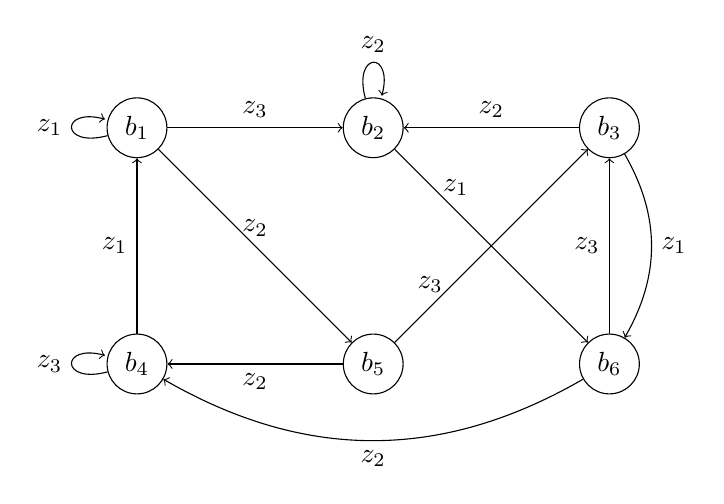
\begin{tikzpicture}
    \node[shape=circle,draw=black] (B1) at (0,0) {$b_1$};
    \node[shape=circle,draw=black] (B2) at (3,0) {$b_2$};
    \node[shape=circle,draw=black] (B3) at (6,0) {$b_3$};
    \node[shape=circle,draw=black] (B4) at (0,-3) {$b_4$};
    \node[shape=circle,draw=black] (B5) at (3,-3) {$b_5$};
    \node[shape=circle,draw=black] (B6) at (6,-3) {$b_6$} ;
    
    \path [->] (B1) edge [loop left] node[left] {$z_1$} (B1);
    \path [->](B1) edge node[above] {$z_3$} (B2);
    \path [->](B1) edge node[above] {$z_2$} (B5);
    \path [->](B4) edge node[left] {$z_1$} (B1);
    \path [->](B2) edge[loop above] node[above] {$z_2$} (B2);
    \path [->](B2) edge node[pos=.2, right] {$z_1$} (B6);
    \path [->](B3) edge node[above] {$z_2$} (B2);
    \path [->](B3) edge [bend left] node[right] {$z_1$} (B6);
    \path [->](B4) edge [loop left] node[left] {$z_3$} (B4);
    \path [->](B5) edge node[pos=.3, left] {$z_3$} (B3);
    \path [->](B5) edge node[below] {$z_2$} (B4);
    \path [->](B6) edge[bend left] node[below] {$z_2$} (B4);
    \path [->](B6) edge node[left] {$z_3$} (B3);
\end{tikzpicture}

